% !TEX root = ../scrreprt/ba_scrreprt_master.tex
% @author Marcel Ruland (2018)

\chapter{Applying \fpmupper}
\label{ch:fpm}
\chapterintro{chapter description goes here}

\section{Method}
\label{sec:fpmmet}
\textit{section description goes here}
%The following subsections begin by introducing the raw data \emph{as-is} and then proceed by describing the process of annotating and evaluating the data, thus going steadily from the most concrete to more and more abstract representations.
%I begin by describing the contents of the video corpus and eventually end with abstract rules\footnote{For the definition of \emph{rule} here, see subsection \ref{ssec:fpmmetapp}.}.

\subsection{The Nature of the Data}
\label{ssec:fpmmetnat}
The corpus is a collection of 10 mother--infant dyads.
Mother and infant were recorded in their own homes during a diaper changing routine.
At the time of recording, infants were 3 months of age, mothers were between 28 and 40 years of age.
This diaper changing routine has several advantages compared to most other activities:
\begin{enumerate}[label={\alph*)}]
	\item it is an activity well-known and familiar to both mother and infant as they both engage in it regularly
	\item mother and infant are in direct interaction with each other for a relatively long period of time
	\item the activity generally takes place without a change of location or a major change of body position/orientation, making recording the data an easier task than it would be for e.g.~a play routine
	\item both mother and infant are free in their expressions; the infant especially is free to make use of body movements and gestures and is not reliant on support from the mother, as might be the case if the infant were sitting
\end{enumerate}
The diaper routine was recorded by two video cameras from two different perspectives, with one camera focused on capturing the mother's behaviour and the other focused on capturing the infant's behaviour.
Figure \ref{fig:rawvid} gives an impression of this raw video data.
For a more detailed description of the setup see \citet[\snum{2.1}]{nomikou_verbs_2017} and \citet[\pnum{115~f.}]{nomikou_language_2011}.\footnote{But note that while the same setup was used, the inclusion or exclusion of groups or individual subjects in the corpus was different due to the different aims of the studies.}
The videos had a mean length of 395~sec (\sd~=~186~sec).

\begin{figure}
	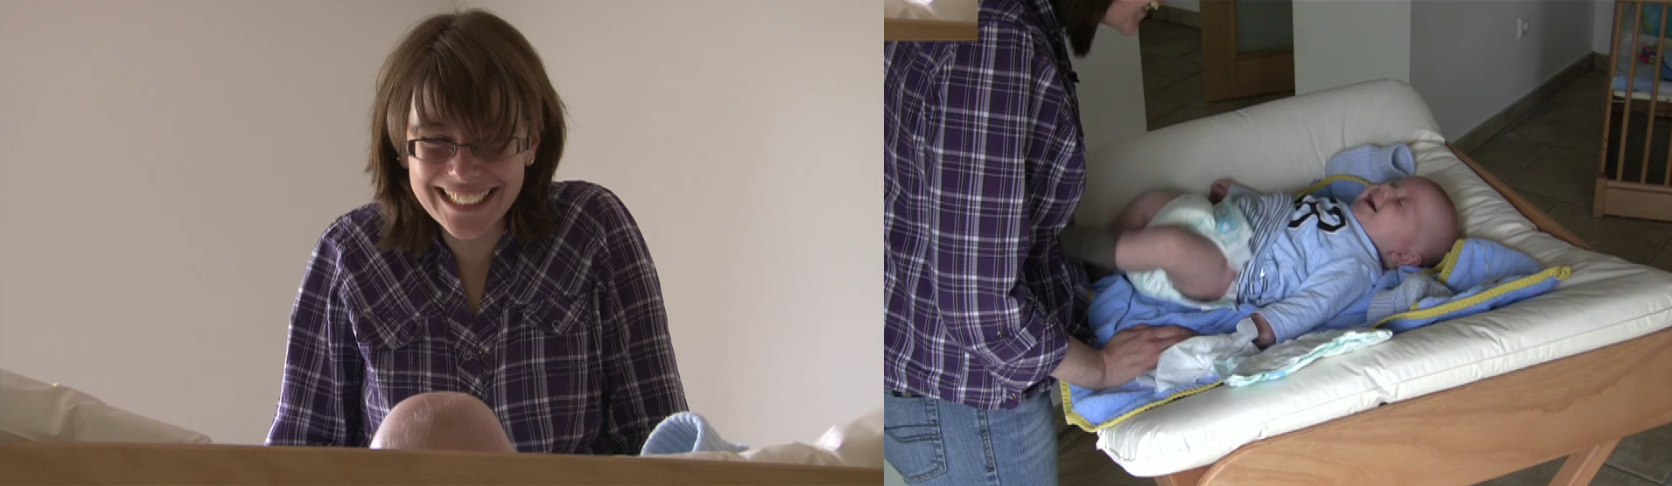
\includegraphics[width=\textwidth]{../aux/img/video_vp_08_compact.png}
	\caption[Screenshot of the raw video data.]{A screenshot of the raw video data showing a mother and her infant during the diaper routine. The left camera captures the mother's behaviour, the right camera captures the infant's behaviour.}
	\label{fig:rawvid}
\end{figure}

\subsection{Annotation of the Videos}
\label{ssec:fpmmetann}
10 kinds of events were hand-coded frame per frame for both mother and infant using the \textsc{elan} software \citep{wittenburg_elan_2006}, yielding an accuracy of \textasciitilde40~\ms\ (videos were recorded with 25 frames per second, therefore a single frame is 40~\ms\ long).
These events were of linguistic, vocal, and visual modality.  % Categories were chosen how? Elaborate here.
They were chosen because, as shown in subsection~\ref{ssec:introrestt}, research has indicated they play a relevant role in early mother-infant interaction.
Table \ref{tab:events} lists all event types.

\begin{table}
	\centering
	\begin{tabularx}{\textwidth}{>{\ttfamily}lX}  % does NOT use \code{}!!
		\toprule
		{\rmfamily Event}	& Explanation \\
		\cmidrule(lr){1-1} \cmidrule(lr){2-2}
		\mosp	& mother speaks \\
		\mogain	& mother gazes at infant \\
		\mogaob	& mother gazing at object, usually diaper but may be any object \\
		\mogaaw	& mother gazes neither at infant nor at object \\
		\mosm	& mother smiles \\
		\midrule
		\invo	& infant vocalises \\
		\cmidrule(lr){2-2}
		\ingamo	& \multirow{4}{*}{\textit{analogous to mother's events}} \\
		\ingaob \\
		\ingaaw \\
		\insm \\
		\bottomrule
	\end{tabularx}
	\caption{Events coded in the data}
	\label{tab:events}
\end{table}

Every annotation contains a start and end time point and therefore also the duration of the respective event.
For example, one specific annotation might say that the mother started smiling at 32.645~\s\ and then smiled continuously until 36.765~\s\, where she stopped smiling again.
This way, sequences as schematised in figure \ref{fig:idealseq} are obtained.
\fpmlabel{A}, \fpmlabel{B}, and \fpmlabel{C} are three different kinds of events; the x-axis represents time.
We see two annotations of type \fpmlabel{A} and \fpmlabel{B} each, as well as a longer annotation of type \fpmlabel{C}.
Those time points that are indicated in black on the x-axis mark the beginning and/or end time point of a specific annotation.
Resulting from this structure, and indicated in parentheses below the grey boxes, are intervals where sets of events are observed.
These sets are the object of interest.
The annotations in the figure show the largest set observable in the indicated intervals, but their subsets are also taken into account.
For example, the set (A,~C) is observed from 4 to 7 and from 8 to 13~\s, because it is a subset of (A,~B,~C).

\begin{figure}
	\centering
	% !TEX root = ../ba_master.tex
% @author Marcel Ruland (2018)
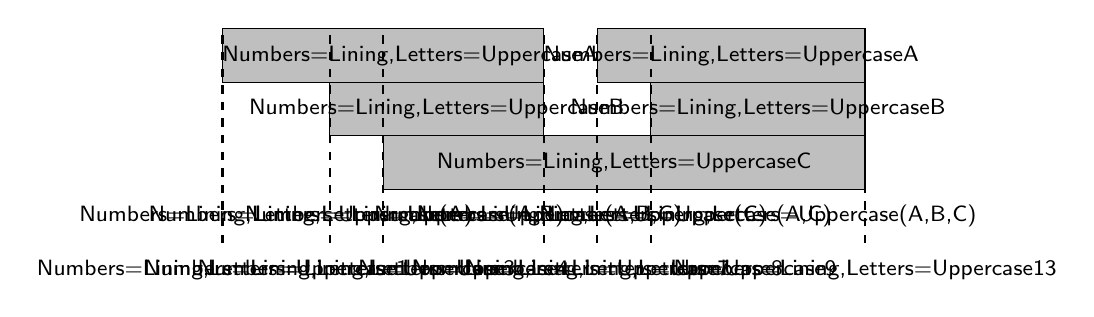
\begin{tikzpicture}[
	scale=0.68,
	every node/.append style={font=\footnotesize\sffamily\addfontfeature{Numbers=Lining,Letters=Uppercase}}]
	% boxes
	\draw [fill=lightgray] (0,4) rectangle (6,5);  % A1
	\node at (3.5,4.5) {A};
	
	\draw [fill=lightgray] (7,4) rectangle (12,5);  % A2
	\node at (9.5,4.5) {A};
	
	\draw [fill=lightgray] (2,3) rectangle (6,4);  % B1
	\node at (4,3.5) {B};
	
	\draw [fill=lightgray] (8,3) rectangle (12,4);  % B2
	\node at (10,3.5) {B};
	
	\draw [fill=lightgray] (3,2) rectangle (12,3);  % C
	\node at (7.5,2.5) {C};
	
	% item sets
	\node at (1,1.5) {(A)};
	\node at (2.5,1.5) {(A,B)};
	\node at (4.5,1.5) {(A,B,C)};
	\node at (6.5,1.5) {(C)};
	\node at (7.5,1.5) {(A,C)};
	\node at (10,1.5) {(A,B,C)};
	
	% time points
	\node at (0,0.5) {1};
	\node at (2,0.5) {3};
	\node at (3,0.5) {4};
	\node at (6,0.5) {7};
	\node at (7,0.5) {8};
	\node at (8,0.5) {9};
	\node at (12,0.5) {13};
	
	% time point lines
	\draw [dashed, thick] (0,1) -- (0,5);
	\draw [dashed, thick] (2,1) -- (2,5);
	\draw [dashed, thick] (3,1) -- (3,5);
	\draw [dashed, thick] (6,1) -- (6,5);
	\draw [dashed, thick] (7,1) -- (7,5);
	\draw [dashed, thick] (8,1) -- (8,5);
	\draw [dashed, thick] (12,1) -- (12,5);
	
	% text representation
%	\node at (6,0) {\code{<(A [1,3]),(A,B [3,4]),(A,B,C [4,7]),(C [7,9])(A,B,C [9,13])>}};
\end{tikzpicture}
	\caption[Sequence schema.]{Schema of an (idealised) sequence.}
	\label{fig:idealseq}
\end{figure}

\paragraph{A note on terminology}
%A mother--infant pair is referred to as a \emph{dyad.}
One individual occurrence of an event is referred to as an \emph{event} (e.g.~the mother smiling from 32.645~\s\ to 36.765~\s\ as described in the previous paragraph).
A certain type of event, such as \code{\mosm}, is called an \emph{event type.}
All events from one mother-child dyad together, regardless of their event type, are called a \emph{sequence.}
Finally, all 10 sequences together are referred to as the \emph{corpus.}


\subsection{Mining Approach}
\label{ssec:fpmmetapp}
\paragraph{Association Rules}
The patterns \citet{rohlfing_multimodal_underreview} mined were association rules of the form \fpmrule{A}{B}, where \fpmset{A} is the \emph{antecedent} and \fpmset{B} the \emph{succedent}.
Antecedent and succedent are sets of events, such that a hypothetical rule may have the form \fpmrule{B,D}{A,C,D}.
An occurrence of a rule represents one of the following two cases:

\begin{enumerate}
	\item the antecedent's start time point lies before that of the succedent.
	\item the antecedent's and succedent's start time points are identical, i.e.\ they begin at the same time.
\end{enumerate}

In addition, rules fulfil the condition that the succedent begins before the antecedent ends, so that there is an overlap.
Referring again to Figure \ref{fig:idealseq}, one can for example observe the rules \fpmrule{A}{B} and \fpmrule{A}{B,C}, because in both cases the antecedent begins before the succedent and the succedent begins before the antecedent ends.
In contrast, there is no occurrence of \fpmrule{B}{A}, because no two observed sets \fpmset{B} and \fpmset{A} fulfil the conditions for a rule.

\paragraph{Adapting the mining scheme}
This scheme can be further adapted to the specific nature of the data.
Given that the data are hand-coded frame per frame, the second condition (antecedent and succedent beginning simultaneously) will in all probability never be true.
The notion of \emph{at the same time} itself is problematic as well.
Humans exhibit a certain reaction time to stimuli, which is always greater than \zero~\ms.
It logically follows that if both mother and infant begin exhibiting a certain event \emph{at the same time,} then one event cannot be a reaction to the other because such a reaction would demand an appropriate reaction time.
Therefore, an interpersonal rule where both events begin at the same time is the result of pure chance.
Capturing chance is not the purpose of rules and, accordingly, such rule occurrences should not be captured at all.
One way of avoiding such rule occurrences is to demand a minimum delay between the beginning of the antecedent and the beginning of the succedent.
In the following paragraph I describe how and why I have chosen to demand a delay of at least 289~\ms\ for rules where the mother's behaviour is the succedent and a delay of at least 850~\ms\ for rules where the infant's behaviour is the succedent.

\paragraph{Choosing appropriate delays}
Human reaction time (henceforth \rt) correlates with a vast variety of factors, among which are intensity, modality, and complexity of the stimulus \citep{brebner_introduction:_1980}, age and gender \citep{der_age_2006}, state of alertness \citep{appelle_simple_1974}, handedness \citep{dane_sex_2003}, and even personality traits \citep{stelmack_personality_1993}.
Quite obviously, many of those traits cannot be determined for the subjects in the corpus used in the present thesis.
However, those factors which are most relevant (namely age of the subject and modality of the stimulus) are both captured in the data and relatively easy to account for.
Regarding modality, variation is very small.
\citet[\pnum{9}]{brebner_introduction:_1980} ascribe variation caused by the modality of the stimulus to ``differences in the peripheral mechanisms rather than in the central processes [of cognition]'' and give average\footnote{The term \emph{average} is used wherever sources do not state whether the value in question is a mean, median, mode, or other measure of centrality.} \rt s of 8--10~\ms\ for acoustic stimuli and 20--40~\ms\ for visual stimuli to reach those central processes.
The resulting difference of 10--32~\ms\ may of course be incorporated in a model of \rt s in the corpus used here, but modelling different \rt s depending on the kind of stimulus complicates the algorithm considerably.
Furthermore, given the small difference caused by stimulus modality, the advantages would be slim.
Therefore the modality of the stimulus has not been incorporated.
Regarding age, mean \rt\ lies  between 1002--1124~\ms\ for infants of age 6--9 months (N~=~24) and between 311--326~\ms\ for adults of age 19--26 years (N~=~11) \citep[\pnum{95}]{leibold_relationship_2002}.%
\footnote{Stimulus was a pure (i.e.~sine wave) tone of 1000~Hertz with loudness ranging from 40--60~dB.
No numerical values given.
Converted from line chart using the Engauge Digitizer software \citep{mitchell_engauge_2002}.
The loudness corresponds to average loudness perceived in conversation \citep[\pnum{32}]{gorne_tontechnik_2006}.}
It would obviously have been desirable to have \rt\ values of 3 month old infants, given that the infants in the  corpus used in the present thesis are 3 months of age.
Unfortunately, such literature does not seem to be available, so the age difference of 3--6 months cannot be avoided for now.
Nevertheless, the important point made is that there \emph{is} a considerable difference in reaction time between infants and adults that must be taken into account.
In my analysis, I therefore capture rules of the sort \fpmtextrule{infant}{mother} (i.e.~mother has to react) if and only if the delay between the start time point of the antecedent and the start time point of the succedent is greater than 289~\ms.
Similarly, rules of the sort \fpmtextrule{mother}{infant} (i.e.~infant has to react) are captured if and only if the delay between the start time point of the antecedent and the start time point of the succedent is greater than 850~\ms.
The values chosen are those given by \citet{leibold_relationship_2002} minus two standard deviations.
This way\dash assuming \rt s to be normally distributed\dash 97.5~\% of \rt s will be longer than the given delays \citep[\pnum{57}]{moore_introduction_2017} and, consequently, only 2.5~\% of \rt s will falsely be sorted out as coincidence.

\paragraph{Reaction time in interaction}
I am well aware that the literature cited with regards to the delays chosen is concerned with \rt\ to general, artificial stimuli and does not consider communication or interaction specifically.
Unfortunately, literature specifically concerned with \rt\ in interaction is virtually inexistent.
There are some indications that it may be faster than general \rt\ \citep{levinson_turn-taking_2016}, but none that it may be slower.
\citepos{levinson_turn-taking_2016} argument deserves further attention.
It unpacks as follows:\showcomment{Has already been explained (how well?) in the section on evolution.}
The fastest \rt\ humans are capable of is around 200~\ms.
This is the \rt\ to a simple start signal with only one possible reaction.
According to Hick's law \citep{hick_rate_1952}, human \rt\ increases logarithmically with the number of available response choices.
Taking vocabulary alone into consideration, languages offer at least 50000 response choices, so that one would expect \rt\ in language to be far above said 200~\ms.
Furthermore, the production of a single primed word takes around 600~\ms, short clauses can take around 1500~\ms.
Despite this, the modal gap between turns is also around 200~\ms.
It follows logically, that production planning must begin before the end of the previous turn.
This gap\dash end of speaker A's turn to beginning of speaker B's turn\dash is the scenario that is currently being discussed in the turn-taking literature \citep[e.g.][among many others]{bogels_listeners_2015,bogels_planning_2018,garrod_use_2015,levinson_timing_2015,riest_anticipation_2015}, but the gap I have applied the minimum delays to is a different one.
Both gaps are schematised in figure \ref{fig:gaps}, with the gap being discussed in the literature on the left side and the gap modelled here on the right side.

\begin{figure}
	\centering
	% !TEX root = ../../scrreprt_figures/ba_scrreprt_figures.tex
% @author Marcel Ruland (2018)
\begin{tikzpicture}[
		every node/.append style={
			font=\sffamily\addfontfeature{Numbers=Lining}
		},
		node distance=2cm and 2cm
	]
%	\draw[help lines, dashed] (0,0) grid (11,4);
	
	% arrows
	\draw[vecArrow] (0,3) to node {\scriptsize\texttt{speech}} (2,3);
	\draw[vecArrow] (2.5,2) to node {\scriptsize\texttt{speech}} (4.5,2);
	\draw[vecArrow] (6.5,3) to node {\scriptsize\texttt{multimodal}} (10.5,3);
	\draw[vecArrow] (7,2) to node {\scriptsize\texttt{multimodal}} (11,2);
	
	% gaps
	\draw[stealth-stealth] (2,1) to node[above] {\tiny gap} (2.5,1);
	\draw[stealth-stealth] (6.5,1) to node[above] {\tiny gap} (7,1);
	
	% dashed lines
	\draw[dashed] (2,0.5) to (2,4);
	\draw[dashed] (2.5,0.5) to (2.5,4);
	\draw[dashed] (6.5,0.5) to (6.5,4);
	\draw[dashed] (7,0.5) to (7,4);
	
	% faces
	\node at (-1,3) (child) {
\includegraphics[height=0.7cm]{../aux/img/child.png}};
	\node at (-1,2) (mother) {
\includegraphics[height=1cm]{../aux/img/woman.png}};
	\node[white] at (child) {\code{A}};
	\node[white] at (mother) {\code{B}};
	
	% annotations
	\node at (2.5,4.5) {gap discussed in the literature};
	\node at (8.5,4.5) {gap modelled in the present thesis};
\end{tikzpicture}
	\caption[Gap in the literature vs gap in the present thesis.]{Comparison of the gap being discussed in the turn-taking literature (left) and the gap being modelled in the present thesis (right).}
	\label{fig:gaps}
\end{figure}

A few important differences between the two gaps must be noted.
Regarding the gap being discussed in the literature, I will refer to \citepos{levinson_turn-taking_2016} paper.
\citeauthor{levinson_turn-taking_2016} is mainly concerned with language only.
Although he does touch on other modalities in his paper, his main line of argumentation is, if at all, only indirectly concerned with multimodality.
In the present scenario, on the other hand, input and output may also be of several non-linguistic modalities, where neither the linguistic cues for an upcoming turn end nor the production times for words and clauses apply.
Secondly, whereas in \citepos{levinson_turn-taking_2016} gap the second speaker is receiving linguistic input that may contain all sorts of clues and cues as to when the ongoing turn will come to an end, this is not (necessarily) the case in the present scenario.
Referring once more to figure \ref{fig:gaps}, one can see that in \citepos{levinson_turn-taking_2016} scenario there is linguistic input immediately preceding the measured gap.
In the present scenario however, this need not be (and most often is not) the case.
There may or may not be input of any modality directly preceding the measured gap but this is not a criterion for the gap itself.
The input preceding the measured gap will be of any modality or combinations of modality.
The influences of this potential multimodal input on the gap are of course there, but it is unclear how big these influences are.
Furthermore, it is likely that they will cancel themselves out in the larger picture.
In short:
\citeauthor{levinson_turn-taking_2016} measures the gap from the \emph{end} of a linguistic turn of speaker \emph{a} to the \emph{beginning} of the following linguistic turn of speaker \emph{b}.
The present thesis measures the gap between the \emph{beginning} of one multimodal event to the \emph{beginning} of another multimodal event.
Therefore, whatever processes might make turn-taking as quick as it is do not apply here.
Some empirical support for this line of argumentation comes from \citet{vanegeren_mother-infant_2001}, who measured a gap similar to the one measured in the present thesis and who found significant results (i.e.~the number of responses to a behaviour being significantly above chance, see also the paragraphs on turn-taking including non-linguistic modalities\showcomment{Has this paragraph maybe been renamed?} in subsection~\ref{ssec:introrestt}) only after a delay of at least 1~\sone, but not before.

It is unlikely that the chosen delays are ideal values.
Consequently, there are two likely possible cases:
The delays chosen are either too long or too short.
If they are too short, then some but not all of the coincidences will be filtered out.
If they are too long, then some real patterns will not be captured but (nearly) all of the coincidences will be filtered out.
It is unlikely, that the delays chosen are exactly right (or that \emph{exactly right} is even a meaningful notion in this context), but for the simple fact that reaction time is always greater than \zero~\ms\ modelling them is a step in the right direction.

For intrapersonal rules only, simultaneous beginnings of antecedent and succedent are meaningful.
Therefore, the delays should not be enforced for intrapersonal rules.
As long as significance is not in the picture, intrapersonal rules without a delay are what the data by \citet{rohlfing_multimodal_underreview} contain.
To introduce significance, many more steps are necessary (see following chapter), which for practical reasons could not be done without a delay for the scope of this thesis.
When discussing the significance of intrapersonal rules, I will refer to the values found when enforcing the shorter delay of 289~\ms.


\section{Metrics}
\label{sec:fpmmetr}
\paragraph{Confidence}
In the literature, the confidence of a rule \fpmrule{A}{B} is commonly defined as \(conf(\mathcal{A\rightarrow B}) = P(\mathcal{B|A})\), the probability of the succedent~\fpmlabel{B}, given the antecedent~\fpmlabel{A} \citep[\pnum{21}]{han_data_2012}.
The definition in the present thesis is somewhat different.\footnote{%
Admittedly, this use of terminology may be confusing. For lack of a better term however, I decided to stick with confidence for the scope of this thesis.}
Here, confidence is defined as
\[conf(\mathcal{A \rightarrow B}) = \frac{d(\mathcal{A \cup B})}{d(\mathcal{A})}\]
where \(d(x)\) is the duration of~\(x\).
The confidence therefore is the duration of the interval where both antecedent and succedent are observed (i.e.~where they overlap) divided by the duration of the interval where the antecedent is observed.
If, in a given occurrence of a rule, we observe the antecedent for 8~\s\ and the overlap of antecedent and succedent is 6~\s, then that occurrence will have a confidence of \(\frac{6~sec}{8~sec} = 0.75\).
Because the interval where both antecedent and succedent are observed cannot be longer than the interval where the antecedent is observed, the confidence has an interval of \((0, 1] = \{x \in \mathbb{R} \mid 0 < x \leq 1 \}\).
A value of \zero\ is not possible because by definition the interval of a rule where both antecedent and succedent are observed is greater than zero.
In other words, the confidence answers to the question:
Over what percentage of the antecedent interval do we observe the succedent?
The infant smiling for a relatively long period of time with the mother eventually joining in with a brief smile herself will result in an occurrence of \fpmtextrule{infant\_smile}{\mosm} with a low confidence close to \zero.
The infant smiling with the mother joining in almost immediately and continuing to smile with the infant for a relatively long period of time will result in an occurrence of \fpmtextrule{infant\_smile}{\mosm} with a high confidence close to 1.
The overall confidence of a rule in a sequence is the mean of all its occurrences' individual confidence values.

It is crucial that the confidence not be misinterpreted as some sort of conditional probability.
A short example will illustrate how different the two metrics behave.
We have a single occurrence of a rule \fpmrule{A}{B}, where we observe the succedent~\fpmlabel{B} over the entire duration of the antecedent~\fpmlabel{A} and \zero\ other occurrences of the antecedent~\fpmlabel{A}.
Both the confidence and the conditional probability will evaluate to 1 in this case.
But if we have not \zero\ but 10 other occurrences of the antecedent~\fpmlabel{A}, the two metrics differ.
The conditional probability will evaluate to \(\frac{1}{10} = 0.1\) because in only 1 of the 10 occurrences of the antecedent we could also observe the succedent.
The confidence however will still evaluate to 1, because the mere observation of the antecedent without observation of the succedent does not count as an occurrence of the rule \fpmrule{A}{B} and therefore is not taken into account by the confidence.
Phrased differently, the confidence is invariant to such sole occurrences of the antecedent.

\paragraph{Total number of occurrences (\noc)}
The total number of occurrences (henceforth \noc) simply counts all occurrences of a given rule in a sequence.
It is a simple yet useful metric that plays an important role in evaluating rules.
If a given rule only occurs only 2--3 times, then this is an indication that coincidence may be playing a relevant role in those 2--3 occurrences.
Still, \noc\ is a metric which is not meaningful alone and must be evaluated together with other metrics, see section \ref{sec:fpmeval}.

\paragraph{Duration}
The duration is another simple yet useful metric.
For a given rule, it is the sum of the durations of all occurrences of that rule.
I.e.~if we have 3 occurrences of a given rule, which are 2, 7, and 4~\s\ long respectively, then that rule's duration evaluates to \(2+7+4=13\)~\s.
The duration of a rule is measured in seconds.

Neither of these three metrics make much sense alone.
A rule may have a high confidence but only show up once, indicating coincidence.
Likewise, a rule may have a long duration but a very low confidence, again indicating coincidence.
A similar case can be made for a rule that appears many times in the sequence but has low confidence and/or duration.
It logically follows that in order to make use of the metrics' power, they must be evaluated in context of each other.

\section{Results}
\label{sec:fpmres}
The results presented in this section are a brief comparison of the rules presented in \citet{rohlfing_multimodal_underreview} with their counterpart when taking \rt s into account.
It is not an extensive discussion, which is reserved for the results in chapter~\ref{ch:sig} after a statistical significance\dash the main aim of this thesis\dash has been established.
I will also intentionally exclude all metrics other than confidence, because confidence is the only metric taken into account in \citet{rohlfing_multimodal_underreview}.
Table~\ref{tab:rtcomp} lists all interpersonal rules explicitly mentioned in \citet{rohlfing_multimodal_underreview} and their confidence values before and after demanding the minimum delays discussed earlier.
For rules with both mother and infant in the succedent, the value given here is the one with the longer delay of 850~\ms.
In the extensive discussion in chapter~\ref{ch:sig}, I will consider values calculated with both the shorter and longer delay for such rules.
Intrapersonal rules are not discussed because reaction time does not play a role here, see end of subsection \ref{ssec:fpmmetapp}.

\newcommand{\asd}{\addfontfeature{Numbers={Monospaced,Lining}}}  % temporary command
\begin{table}  % Why is there an indent at the beginning of a rule?
	\begin{tabularx}{\textwidth}{>{\sffamily\addfontfeature{Numbers=Lining,Letters=Uppercase}}cX>{\asd}l>{\asd}l>{\asd}r@{.}>{\asd}l}
		\toprule
		&& \multicolumn{4}{c}{{\sffamily confidence}} \\
		\cmidrule(lr){3-6}
		\# & \multicolumn{1}{c}{{\sffamily rule}} & {\sffamily no \rt} & {\sffamily \rt} & \multicolumn{2}{l}{\sffamily change}\\
		\midrule
		(5)  & \fpmtextrule{\mosp, \mogain}{\ingamo} & 0.62 & \textsc{na} \\
		(6)  & \fpmtextrule{\mogain}{\ingamo} & 0.63 & 0.62 & --0&01\\
		(7)  & \fpmtextrule{\ingamo}{\mosp} & 0.84 & 0.42 & --0&42\\
		(8)  & \fpmtextrule{\ingamo}{\mogain} & 0.65 & 0.63 & --0&02\\
		(9)  & \fpmtextrule{\ingamo}{\mosp, \mogain} & 0.64 & \textsc{na} \\
		(10) & \fpmtextrule{\mosp, \mogaaw, \ingaob}{\mosm} & 0.50 & \textsc{na} \\
		(11) & \fpmtextrule{\mogaaw, \ingaob}{\mosp, \mosm} & 0.50 & \textsc{na} \\
		(12) & \fpmtextrule{\ingaob}{\mogaob} & 0.49 & 0.49 & 0&00\\
		(13) & \fpmtextrule{\mosp, \mosm, \mogaaw, \ingaaw}{\insm} & 0.61 & \textsc{na} \\
		(14) & \fpmtextrule{\mosm, \mogaaw, \ingaaw}{\insm} & 0.61 & \textsc{na} \\
		(15) & \fpmtextrule{\mogain, \ingamo, \mogaob}{\invo} & 0.44 & \textsc{na} \\
		(16) & \fpmtextrule{\mogain, \ingamo, \mogaob}{\mosp, \invo} & 0.44 & \textsc{na} \\
		(17) & \fpmtextrule{\mosp, \ingamo, \invo, \insm}{\mogain} & 0.37 & \textsc{na} \\
		\bottomrule
	\end{tabularx}
	\caption[Rules in \citet{rohlfing_multimodal_underreview} with \rt.]{Rules mentioned in \citet{rohlfing_multimodal_underreview} and their confidence values without and with \rt. A rule's index in parentheses is identical to that rule's index in \citet{rohlfing_multimodal_underreview}.}
	\label{tab:rtcomp}
\end{table}

Going back to table~\ref{tab:rtcomp}, the first thing that strikes the eye, is that out of the 13 interpersonal rules discussed in \citet{rohlfing_multimodal_underreview}, 9 have not been observed when taking \rt\ into account, indicating that for every occurrence of these rules the beginning of the succedent was less than the respective \rt\ after the antecedent.
We also see differences in confidence, shown in the right-most column of the table.
While most of these differences change little about the rule's interpretation, there is one substantial difference visible.
The confidence of rule (7) drops by half, indicating that some of the rule's occurrences may have been coincidence.
This is in line with a peculiarity of the data set:
Mothers' speech is observed for a majority of the time, making other events incidentally coinciding with it likely.

Finally, rules (15) and (16) are unusual.
Their (identical) antecedents contain both the event \mogain\ and the event \mogaob.
Such an interval suggests that the mother look at her baby and at an object \emph{at the same time,} which of course is not possible.
A closer look at the data reveals that both rules only occur a single time and only for 0.45~\s.
In fact, both rules are derived from the same 0.45~\s\ interval in the data (the succedent of rule (15) is a subset of the succedent of rule (16)).
The most likely reason for this isolated occurrence of an impossible antecedent is a simple coding error.
